\documentclass[]{article}
\usepackage{lmodern}
\usepackage{amssymb,amsmath}
\usepackage{ifxetex,ifluatex}
\usepackage{fixltx2e} % provides \textsubscript
\ifnum 0\ifxetex 1\fi\ifluatex 1\fi=0 % if pdftex
  \usepackage[T1]{fontenc}
  \usepackage[utf8]{inputenc}
\else % if luatex or xelatex
  \ifxetex
    \usepackage{mathspec}
  \else
    \usepackage{fontspec}
  \fi
  \defaultfontfeatures{Ligatures=TeX,Scale=MatchLowercase}
\fi
% use upquote if available, for straight quotes in verbatim environments
\IfFileExists{upquote.sty}{\usepackage{upquote}}{}
% use microtype if available
\IfFileExists{microtype.sty}{%
\usepackage{microtype}
\UseMicrotypeSet[protrusion]{basicmath} % disable protrusion for tt fonts
}{}
\usepackage[left=1.5in,right=1.5in,top=1.5in,bottom=1.5in]{geometry}
\usepackage{hyperref}
\PassOptionsToPackage{usenames,dvipsnames}{color} % color is loaded by hyperref
\hypersetup{unicode=true,
            colorlinks=true,
            linkcolor=blue,
            citecolor=Blue,
            urlcolor=Blue,
            breaklinks=true}
\urlstyle{same}  % don't use monospace font for urls
\usepackage{longtable,booktabs}
\usepackage{graphicx,grffile}
\makeatletter
\def\maxwidth{\ifdim\Gin@nat@width>\linewidth\linewidth\else\Gin@nat@width\fi}
\def\maxheight{\ifdim\Gin@nat@height>\textheight\textheight\else\Gin@nat@height\fi}
\makeatother
% Scale images if necessary, so that they will not overflow the page
% margins by default, and it is still possible to overwrite the defaults
% using explicit options in \includegraphics[width, height, ...]{}
\setkeys{Gin}{width=\maxwidth,height=\maxheight,keepaspectratio}
\IfFileExists{parskip.sty}{%
\usepackage{parskip}
}{% else
\setlength{\parindent}{0pt}
\setlength{\parskip}{6pt plus 2pt minus 1pt}
}
\setlength{\emergencystretch}{3em}  % prevent overfull lines
\providecommand{\tightlist}{%
  \setlength{\itemsep}{0pt}\setlength{\parskip}{0pt}}
\setcounter{secnumdepth}{0}
% Redefines (sub)paragraphs to behave more like sections
\ifx\paragraph\undefined\else
\let\oldparagraph\paragraph
\renewcommand{\paragraph}[1]{\oldparagraph{#1}\mbox{}}
\fi
\ifx\subparagraph\undefined\else
\let\oldsubparagraph\subparagraph
\renewcommand{\subparagraph}[1]{\oldsubparagraph{#1}\mbox{}}
\fi

%%% Use protect on footnotes to avoid problems with footnotes in titles
\let\rmarkdownfootnote\footnote%
\def\footnote{\protect\rmarkdownfootnote}

%%% Change title format to be more compact
\usepackage{titling}

% Create subtitle command for use in maketitle
\newcommand{\subtitle}[1]{
  \posttitle{
    \begin{center}\large#1\end{center}
    }
}

\setlength{\droptitle}{-2em}

  \title{}
    \pretitle{\vspace{\droptitle}}
  \posttitle{}
    \author{}
    \preauthor{}\postauthor{}
    \date{}
    \predate{}\postdate{}
  
\usepackage{fontspec}
\setmainfont{Times}
\usepackage{setspace}
\usepackage{algorithm2e}

\begin{document}

\newcommand{\smallfont}[1]{{%
  \fontsize{10pt}{12pt}\normalfont #1%
}}
\newcommand{\midsmallfont}[1]{{%
  \fontsize{15pt}{17pt}\normalfont #1%
}}
\newcommand{\normfont}[1]{{%
  \fontsize{20pt}{24pt}\normalfont #1%
}}
\newcommand{\midfont}[1]{{%
  \fontsize{24pt}{28pt}\normalfont #1%
}}
\newcommand{\bigfont}[1]{{%
  \fontsize{30pt}{36pt}\normalfont #1%
}}

\leavevmode
\newline
\newline
\newline
\newline
\newline
\newline
\newline
\newline
\newline
\newline
\newline
\newline

\begin{center}
\bigfont{Scalable Inference for}

\midfont{Gaussian Hierarchical Models} 
\end{center}

\vspace{2.0cm}

\begin{center}
\large Master Thesis \\ Kwa Jie Hao
\end{center}

\vspace{0.5cm}

\begin{spacing}{1.0}
\begin{center}
\large Supervisors: \\ Prof. Omiros Papaspiliopoulos (UPF) \\ Prof. Giacomo Zanella (Bocconi)
\end{center}
\end{spacing}

\vspace{2.0cm}

\begin{center}
\normalsize Submitted in partial fulfillment of the requirements \\ for the Master's Degree in Data Science \\ at the Barcelona Graduate School of Economics, 2018
\end{center}

\newpage

\midfont{1. Introduction} \newline

Hierarchy is an organization of items into different levels based on a
certain logic, such that items in a set are linked directly either to
other items above and below it to produce an overall structure for all
the items in a given set. For better or for worse, hierarchy is
frequently observed both in human society and its institutions as well
as in nature (such as dominance hierarchies in animal packs).
Accordingly, much of the data that is available for statistical analysis
can be modeled in a multilevel manner. For example, data about the
performance of individuals in a company can be modeled as a 2-level
hierarchy begining with the entire company, followed by departments,
sub-teams within each department, and finally individuals. The
frequently superior performance of multilevel\footnote{For the purposes
  of this paper, the reader should take the terms ``multilevel'' and
  ``hierarchical'' to mean the same thing.} modeling (Gelman, 2006) in
different contexts affirms the validity of understanding the world
around us in a hierarchical manner.

This paper will attempt to highlight the advantages of hierarchical
models and study scalable methods for inference on Gaussian hierarchical
models. The aims of this thesis are three-fold. Firstly, it will explore
the formulation of posterior inference of Gaussian hierarchical models
using Gaussian simulation as a linear algebra problem which can be
solved with efficient sparse linear algebra methods. The second goal is
to provide tools for inference for Gaussian hierarchical models in the
form of an R package. Finally, this paper will analyze the performance
of existing linear algebra packages \emph{spam} and \emph{Matrix} in
obtaining the optimal fill-in of the cholesky factor.

For the purposes of this paper, all observations are taken to be 0. The
main issue of concern here is computational efficiency. This assumption
is a valid one since performance of the methods considered in this paper
depend only on the structure of the covariance alone, which remains
unaffected by the specific values of the observations for Gaussian
hierarchical models. \newline \newline \newline

\midsmallfont{1.1 Notation} \newline

To keep the equations short and readable, I have adopted the following
notation for hierarchical variables. The root variable is denoted as
\(\beta\).

For variables at the first level,
\[\beta_{1:I} = \beta_1, \beta_2, ..., \beta_I\]

At the second level,
\[\beta_{1:I,1:J} = \beta_{11}, \beta_{12}, ..., \beta_{21}, \beta_{22}, ...,\beta_{IJ}\]
And so on for deeper levels. \newline \newline \newline

\newpage

\midfont{2. Gaussian Hierarchical Models} \newline \newline \newline
\midsmallfont{2.1 Advantages of Hierarchical Modeling} \newline 

Since the structure of many institutions or objects being studied is
either explicitly or implicitly hierarchical, hierarchical models can
more accurately capture the multilevel dynamics of the data on these
objects. The use of hierarchical models allows us to fit a regression
model at an individual level while also simultaneously explain the
systematic variation at higher grouping levels (Gelman, 2006). This
allows specific traits of different groups at different levels to be
identified and makes it easier to characterize these groupings while
also accounting for individual variation within groups, making
inferences from multilevel models more reasonable. Models which utilize
complete pooling give identical estimates to all sub-groups, which is
not ideal especially when there is substantial variation between
sub-groups, whereas for models where no pooling is done, the model is
likely to overfit the data and be more susceptible to outliers.

On an anecdotal level, this is easy to understand: A person from
Catalonia is likely to have certain traits which are unique to Catalans
but also have in common traits with Spanish people in other regions
which are characteristic of people living in Spain.

Furthermore, hierarchical models offer a framework to combine
information across units (such as individuals or counties) and have been
empirically shown to provide well-calibrated and more accurate
predictions of observable outcomes (Draper, 1995) by using
cross-validation (Gelman, 2006), especially when predicting group
averages.

Finally, under certain conditions (such as conditional conjugacy of the
prior and posterior distributions), hierarchical models allows us to
utilize Bayesian statistical tools and techniques which allows us to
learn from the data at different levels and conduct sampling-based
inference. The multilevel structure of these models allow us to organize
inference into a directed acyclic graph such that the observations at
the bottom layer are the leaves, and the top layer being the
hyperparameters, with intermediate parameters in the levels in between.
Such a graph is easy to sample conditionally from, which can be done
simply by calculating posterior distributions. This allows us to sample
both exactly (using the precision matrix) and approximately (through
Markov Chain Monte Carlo methods like Gibbs sampling). It is this
quality precisely which will be exploited and studied in this paper.

\begin{center}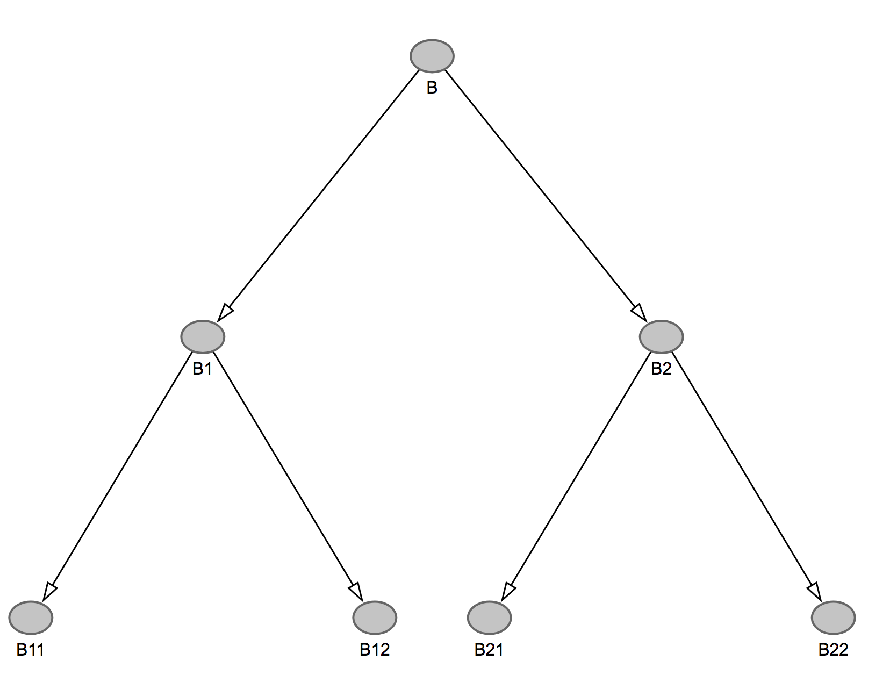
\includegraphics[width=200bp]{Paper_files/figure-latex/example-1} \end{center}

\begin{center} \smallfont{Figure 1. A simple hierarchical model generated using DAGitty. Sampling is easily done by sampling first from the leaves (B11, B12 ...) and then sampling conditional on the previously obtained samples.}  \end{center}

\vspace{0.5cm}

\midsmallfont{2.2 Posterior inference on Gaussian hierarchical models}
\newline 

The rest of the paper will focus specifically on tree-structured
hierarchical models where each parameter follows a Gaussian
distribution. Tree-structured Gaussian hierarchical models depends only
on the covariance of the parameters involved and not the mean, and thus
allows exact sampling to be conducted and studied. It is also assumed
that the variance of parameters within the same level are the same since
the focus is on scalable inference, which is unaffected by specific
values of the variances. Thus, all variance parameters are set to 1 and
the mean for the root parameter \(\beta\) is set to 0 for the rest of
this paper. For now, the focus of this paper is restricted to a 2-level
multivariate Gaussian model with full-centered parameterizations (that
is, the number of children nodes for each node in the first level is the
same, resulting in a symmetric tree structure) (Zanella, Roberts, 2017).
For i = 1, \ldots{}, I and j = 1,\ldots{},J,

\[\beta \sim  N( \mu, \tau) \;\;\;- (2.1)\]

\[\beta_i \;|\; \beta \sim N( \beta, \tau_a) \;\;\; - (2.2)\]
\[\beta_{ij} \;|\; \beta_i \sim N( \beta_i, \tau_b) \;\;\; - (2.3)\]
\[y_{ij} \;|\; \beta_{ij} \sim N( \beta_{ij}, \sigma^2) \;\;\; - (2.4)\]

where it is assumed that the variances for each level,
\(\tau, \tau_a, \tau_b, \sigma^2\), are the same for variables within
the same level, and that there is only one observation \(y_{ij}\) for
each parameter \(\beta_{ij}\). Extension to a 3- or higher level model
is simple and can be found in Appendix A1.

For posterior inference, it is useful to first look at the joint
posterior distribution of the parameters conditional on the observations
(and also conditional on the variance parameters which have been set to
1). This is easy to calculate since the joint distribution is Gaussian.
Let \(\boldsymbol{\beta}\) represent
\((\beta, \beta_1, ..., \beta_I, \beta_{11}, ..., \beta_{IJ})\), let
\(\boldsymbol{y}\) represent \((y_{11}, ..., y_{IJ})\). The posterior
density \(P(\boldsymbol{\beta} \; | \; \boldsymbol{y})\) is given by:

\[
\begin{aligned} 
P(\boldsymbol{\beta} \;|\;\boldsymbol{y}) &= \frac{P(\boldsymbol{y} \;|\;\ \boldsymbol{\beta}) P(\boldsymbol{\beta})}{P(\boldsymbol{y})} \\
&\propto P(\boldsymbol{y}\;|\; \boldsymbol{\beta}) P(\boldsymbol{\beta})\;\;\; - (2.5)
\end{aligned}
\]

Note that since the model in question is a tree graph such that each
node is connected to, and thus by d-separation, dependent only on its
parent node and child nodes, for any given \(i,j\):

\[P(y_{ij} \;|\; \boldsymbol{\beta}) = p(y_{ij} \;|\; \beta_{ij}) \;\;\; - (2.6)\]
This factorization can be repeated for \(P(\boldsymbol{\beta})\) until
the factorization in (2.7) is obtained. Since the variables are
Gaussian, this equation can be expressed explicitly using the formula
for Gaussian densities:

\[ 
\begin{aligned}
P(\boldsymbol{\beta} \;|\;\boldsymbol{y}) &\propto P(\boldsymbol{y}\;|\; \boldsymbol{\beta}) P(\boldsymbol{\beta}) \\  &=  P(\beta) \prod_{i} P(\beta_i \;|\; \beta) \prod_{i,j}P(\beta_{ij} \;|\; \beta_i)  \prod_{i,j}P(y_{ij} \;|\; \beta_{ij}) \\
&\propto \exp\{-\frac{1}{2\sigma^2}\ \sum_{i,j} (y_{ij}-\beta_{ij})^2 - \frac{1}{2\tau_b}\sum_{i,j} (\beta_{ij}-\beta_{i})^2 - \frac{1}{2\tau_a} \sum_{i} (\beta_{i}-\beta)^2 -\frac{1}{2\tau}(\beta - \mu)^2 \}\;\;\; - (2.7)\\
&\propto \exp\{-\frac{1}{2} \boldsymbol{\beta^{T}} Q \boldsymbol{\beta}\} \;\;\; - (2.8)
\end{aligned}
\]

Equation (2.7) is useful because the entries of the precision matrix of
the posterior distribution can be easily calculated from it (Appendix
A2).

Traditional inference using linear algebra methods become infeasible
when the number of parameters involved grow to extremely large numbers.
To obtain a sample \(\boldsymbol{V}\) from a \(m\)-dimensional
multivariate Gaussian such that
\(\boldsymbol{V} \sim N(\boldsymbol{\mu},\boldsymbol{\Sigma})\), one
first samples from a multivariate standard normal
\(\boldsymbol{z} \sim N(0,I_m)\), multiply it by the cholesky factor
\(\boldsymbol{\tilde{L}}\) of the covariance matrix , and add the mean
of the parameters \(\boldsymbol{\mu}\).

\[\boldsymbol{V} = \boldsymbol{\mu} + \tilde{L} \boldsymbol{z} \;\;\; - (2.9)\]

where \(\tilde{L}\tilde{L^T} = \Sigma\). In sampling these parameters,
one would need to compute the cholesky factor of the covariance matrix,
which require \(O(n^3)\) flops where \(n\) is the total number of
parameters for a dense matrix. Alternatively, if the covariance matrix
is not known but the precision matrix is known, one can generate samples
by using the cholesky factor \(\boldsymbol{L}\) of the precision matrix
\(\boldsymbol{Q}\).

\[\boldsymbol{V} = \boldsymbol{\mu} + L^{-T} \boldsymbol{z} = \boldsymbol{\mu} + \boldsymbol{v} \;\;\; - (2.10)\]
where \(LL^T = \boldsymbol{Q}\). This still requires \(O(n^3)\) flops to
decompose a dense matrix (the cholesky decomposition is the limiting
factor as it is quick to solve \(L^T \boldsymbol{v} = \boldsymbol{z}\)
since L is lower triangular).

However, more efficient methods are available when the model in question
is a tree-structured hierarchical model. For such models, the precision
matrix of the parameters is sparse due to the conditional independence
structure of the parameters which arises from the tree-structure of the
model. This sparsity can be exploited to speed up the matrix
factorization step to require only \(O(n)\) flops (Rue, Held, 2002). The
issue of posterior inference on Gaussian hierarchical models thus
becomes a linear algebra problem which can be solved with sparse linear
algebra techniques. \newline \newline \newline

\midsmallfont{2.3 Sparsity} \newline 

The sparsity of the precision matrix for Gaussian hierarchical models
follows directly from the conditional independence properties of the
model. To illustrate this more clearly, it is useful to consider the
graph for Gaussian hierarchical models. Since each of the parameters
follows a Gaussian distribution, the graph for tree-structured Gaussian
hierarchical models can be represented as a Gaussian Markov Random Field
(or GMRF) (Rue, Held, 2002). Note that due to the tree structure of the
model, the structure of the graph is the same whether it is represented
as a GMRF or a DAG. The set of parameters,
\(\boldsymbol{x} = (x_1, ..., x_n)\), is a GMRF with respect to \(G\) if
\(G = (V,E)\) where \(V = \{1,...,n\}\) is the set of (labeled) nodes
which represent the parameters in the graph, and \(E\) is the set of
edges which connect the nodes such that there is no edge between node
\(i\) and node \(j\) if and only if:

\[x_i \; \perp \; x_j \;|\; \boldsymbol{x}_{-\{ij\}} \;\;\; - (2.11)\]

where \(\boldsymbol{x_{-\{ij\}}} = \boldsymbol{x_{-\{i,j\}}}\). Equation
(2.11) is also known as the pairwise Markov property. Using this
information, the following result can be obtained (refer to appendix
A3). For \(i \neq j\),

\[x_i \; \perp \; x_j \;|\; \boldsymbol{x}_{-\{ij\}} \iff Q_{ij}=0 \;\;\; - (2.12)\]

where \(\boldsymbol{Q}\) is the precision matrix of the parameters. This
says that two parameters \(x_i\) and \(x_j\) are independent conditional
on the other parameters if and only if the term in the \(i^{\text{th}}\)
column and \(j^{\text{th}}\) row of the precision matrix is 0. Thus, for
a given precision matrix, the conditional independence properties of the
graph can be deduced. More importantly, for a given graph \(G\), this
result makes it easy to determine where the zero and non-zero elements
of the precision matrix are and to calculate and store only the non-zero
values.

In this framework, the precision matrix of Gaussian hierarchical models
tend to be very sparse. The hierarchical structure of the model means
that each node in the model is dependent only on its parent or child
node. Since any two nodes which do not have an edge between them has a
conditional precision of 0, most of the entries in the precision matrix
are 0. This permits the use of sparse linear algebra algorithms for more
efficient cholesky factorization. \newline \newline \newline

\midsmallfont{2.4 Sparse linear algebra methods} \newline 

To sample from the model, the cholesky factor of the precision matrix
needs to be computed, as seen in equation (2.10). As mentioned before,
cholesky decomposition of a dense matrix requires \(O(n^3)\) flops but
with the sparse precision matrix of Gaussian hierarchical models, the
following method can be used to reduce the complexity to at best
\(O(n)\) flops by making use of the sparsity of the graph to find zeros
in the cholesky factor.

Let \(L\) be the cholesky triangle of \(\boldsymbol{Q}\), and define for
\(1\leq i \leq j \leq n\) the set
\(F(i,j) = \{i+1, ..., j-1, j+1, ..., n\}\), or the \emph{future} of
\(i\) except \(j\). Then we have a similar result (refer to Appendix
A4):

\[x_i \; \perp \; x_j \;|\; \boldsymbol{x}_{F(i,j)} \iff L_{ji}=0 \;\;\; - (2.13)\]
If \(F(i,j)\) separates node \(i<j\), then
\(x_i \; \perp \; x_j \;|\; \boldsymbol{x}_{F(i,j)}\) and \(L_{ij}=0\).
However, if \(F(i,j)\) does not separate the two nodes, then a
calculation needs to be carried out to determine the value of
\(L_{ij}\), which may or may not be zero. In other words, if we can
verify that \(L_{ij}\) is 0, then we do not have to compute it. Applying
the global Markov property (Appendix A5), this verification can be done
by ensuring that the future set \(F(i,j)\) separates \(i\) and \(j\) in
the graph \(G\) that defines the GMRF where \(i<j\).

Therefore, to minimize computation, it is desirable to find a
permutation such that
\(x_i \; \perp \; x_j \;|\; \boldsymbol{x}_{F(i,j)}\) for as many values
of \(i\) and \(j\) as possible. It is the conditional independence
structure of the graph which determines which nodes are connected to
which, and therefore which nodes are separated by which, which
determines \(F(i,j)\), thus affecting whether or not \(L_{ij}=0\). The
more zeros we have in our cholesky factor \(\boldsymbol{L}\), the less
calculations needed to obtain the cholesky factor since only the
non-zero elements are calculated.

Using again the global Markov property and equation (2.13) (maybe can be
explained more in the appendix), \(L\) is more or equally dense than the
lower triangular part of \(\boldsymbol{Q}\), which has \(n_Q = n-1\)
entries (it is easy to see why the precision matrix has \(n-1\) entries
from equation (2.12)). In other words, the number of non-zero elements
in the cholesky factor, \(n_L\), is always greater than or equal to
\(n_Q\). The efficiency of the cholesky factorization can thus be
measured by the fill-in ratio \(\frac{n_L}{n_Q}\) since the closer the
fill-in ratio to 1, the less non-zero elements need to be calculated.
Optimal efficiency is thus achieved when the fill-in ratio is 1 and only
\(n-1\) entries need to be calculated, which is linear in the number of
nodes.

Therefore, the ordering of individual nodes are important as they can be
re-ordered so that overall, as many node pairs (\(i\),\(j\)) as possible
are separated by \(F(i,j)\) for any \(i\) and \(j\), leading to lower
\(n_L\) and greater computational gains. In general, it is beneficial
for nodes that are connected to many other nodes to have higher numbers,
so that conditional independence between any 2 nodes given the set
\(F(i,j)\) is more likely. For instance, if all nodes depend on node 1,
for any \(1 < i < j \leq n\), the future set \(F(i,j)\) will never
separate \(i\) and \(j\) as every node is connected to node 1, leading
to maximal fill-in. This is illustrated in Figure 2 below. This line of
reasoning leads to the concept of nested dissection (Rue, Held, 2002).

\begin{center}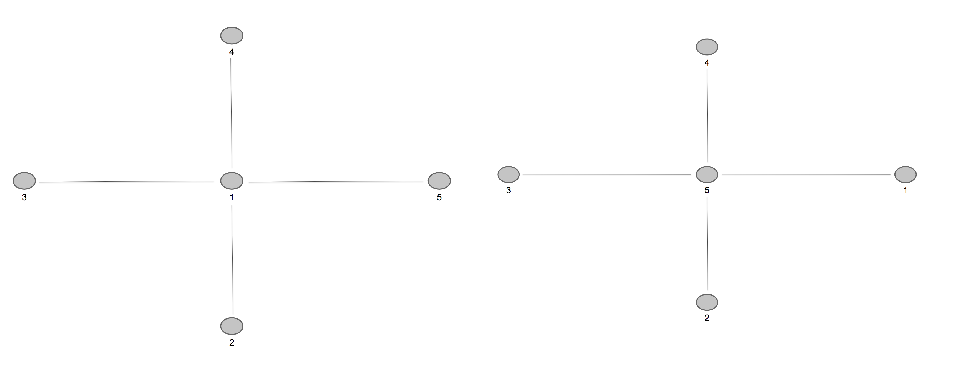
\includegraphics[width=400bp]{Paper_files/figure-latex/future-1} \end{center}

~~~~~~~~~~~~~~~~~~~~~~~~~~~~~~~~~~~~~ (a)
~~~~~~~~~~~~~~~~~~~~~~~~~~~~~~~~~~~~~~~~~~~~~~~~~~~~~~~~~~~~~~~~~~~~~~~~~~~~
(b)

\begin{center} \smallfont{Figure 2. Two graphs which illustrate the importance of ordering of nodes to computational efficiency. In graph (a), every node is connected to node 1 and only node 1, making it in the future set of every node. Thus, fill-in is maximal and the cholesky factorization for its precision matrix is $O(n^3)$. However, in graph (b), every node is connected to node 6 and only in node 6. It is thus in none of the future sets of any of the other nodes, making fill-in minmal and reducing complexity to $O(n)$}  \end{center}

\vspace{0.6cm}

Permutation of the precision matrix can be done by finding a permutation
matrix \(\boldsymbol{P}\) such that
\(\boldsymbol{i}^p = \boldsymbol{Pi}\) where
\(\boldsymbol{i} = \{1,..,n\}^T\) is the original ordering of the nodes
and \(\boldsymbol{i}^p\) is the new ordering. \(\boldsymbol{P}\) is then
chosen such that the resulting permuted precision matrix
\(\boldsymbol{Q}^p = \boldsymbol{PQP}^T\) leads to a reduction in
fill-in for the cholesky factor. \(\boldsymbol{P}\) can be chosen based
on the principles of nested dissection. By selecting a small set of
nodes whose removal divides the graph into two disconnected subgraphs of
almost equal size and give them the highest numbers, re-ordering the
nodes in each of the subgraphs, and repeating the same procedure to the
rest of the nodes in each of the subgraphs. On average, algorithms based
on nested dissection ordering require \(O(n^{3/2})\) flops and gives
\(O(n logn)\) fill-ins (George, Liu, 1981). However, for graphs with
cleaner structures such as Gaussian hierarchical models, optimal fill-in
and faster performance is possible. \newline \newline \newline

\midsmallfont{2.5 Gibbs Sampler} \newline 

Efficient performance of above method is reliant on finding the right
permutation matrix which can be hard to do without the right algorithm.
The alternative to exact inference with sparse linear algebra methods is
approximate inference belonging to the class of Monte Carlo Markov Chain
methods such as the Gibbs sampler. The Gibbs sampler relies on
calculating full conditionals of each parameter and sampling based on
those conditionals (Appendix A6). In particular, the graph structure of
the hierarchical model makes sampling from conditionals easily by
sampling firstly from the leaves of the graph and then sampling upwards
based on samples at lower levels. For a long enough time period, samples
drawn from the Gibbs sampler with subsampling (since subsequent samples
are highly correlated) resemble independent draws from the target
distribution. The complexity is linear in the number of parameters and
thus competitive with the sparse linear algebra methods. In particular,
the Gibbs sampler used here is based off GS(0,0) in Zanella, Roberts
(2017). The algorithm for the Gibbs sampler for a centered 2-level
Gaussian hierarchical model is as follows:

\begin{algorithm}[H]
 Initialize $\beta^{* (0)} = \beta^{(0)}, \beta_1^{(0)}, ..., \beta_I^{(0)}, \beta_{11}^{(0)}, ..., \beta_{IJ}^{(0)}$ randomly\;
 \For{t = 1 to T}{  
  \For{i = 1 to I}{
    \For{j = 1 to J}{
    Sample $\beta_{ij}^{(t)} \;|\; \beta^{(t-1)}, \;\beta_{1:I}^{(t-1)}$\;
    }{
    Sample $\beta_{i}^{(t)} \;|\; \beta^{(t-1)}, \;\beta_{i, 1:J}^{(t)}$
    }
  }
  Sample $\beta^{(t)} \;|\; \beta_{1:I}^{(t)}, \;\beta_{1:I,1:J}^{(t)}$   
 }
 \caption{Gibbs Sampler}
\end{algorithm}

\vspace{1.0cm} \newpage
\midfont{3. Experiments} \newline \newline \newline
\midsmallfont{3.1 ghInf} \newline 

The R package \emph{ghInf} was created to aid with the simulations
conducted in this paper. \emph{ghInf} provides multiple tools for
inference with Gaussian hierarchical models. This includes functions
which calculate the precision matrix for both centered and uncentered
parametrizations of 2- and 3-level Gaussian hierarchical models and a
Gibbs sampler for centered 2- and 3-level models. The code can be found
here on \href{https://github.com/kwajiehao/ghInf}{Github}.
\newline \newline \newline

\midsmallfont{3.2 \*Matrix\* and \*spam\* packages} \newline 

The \emph{Matrix} and \emph{spam} packages are linear algebra packages
for R. \emph{Matrix} is a larger package with methods for a wide variety
of functions which make use of linear algebra libraries such as BLAS
(Basic Linear Algebra Subroutines), Lapack (dense matrix), CHOLMOD and
Csparse (sparse matrix) routines (Maechler, Bates, 2006). On the other
hand, \emph{spam} is a more focused sparse matrix R package which an
emphasis on Monte Carlo Markov Chain methods for Gaussian Markov Random
Fields (Furrer, Sain, 2010). The main function of interest in both
packages is the cholesky decomposition function, \emph{chol}, which is
important in sampling-based inference of Gaussian hierarchical models.
The \emph{chol} function in \emph{Matrix} uses CHOLMOD (Davis, 2009), a
sparse supernodal Cholesky factorization routine, whereas \emph{spam}
uses the block sparse Cholesky algorithm (a supernodal left-looking -
constructing the lower triangular factor \(\text{R}^{\text{T}}\)
column-wise - Cholesky factorization) of Ng and Peyton (1993). For the
purposes of this paper, the differences in the methods is not important
since both routines return the same cholesky factor. This is because the
precision matrix is positive definite and the cholesky factor of a
positive definite matrix is unique.

Cholesky decomposition functions, especially for sparse matrices, often
use permutation algorithms to permute the rows and columns of a matrix
to reduce the fill-in and thus make computation more efficient. The
\emph{spam} package uses the multiple minimum degree algorithm (MMD)
(George, Liu, 1989) by default to permute the matrix whereas the
\emph{Matrix} package uses the approximate minimum degree algorithm
(AMD) (Amestoy, Davis, Duff, 1996). Both algorithms seek to directly
reduce the fill-in of the cholesky factor as opposed to bandwith
reduction methods. The difference between AMD and MMD are highly
technical and irrelevant to the results of this paper.

Both \emph{Matrix} and \emph{spam} packages have cholesky decomposition
functions which allow for pivot = FALSE. This means that the function
attempts to compute the cholesky factor without using the AMD or MMD
permutation algorithm. This allows performance comparisons to be made
between the fill-in obtained using each package's respective permutation
algorithm versus without to illustrate the importance of row and column
permutation in factorizing sparse matrices. \newline \newline \newline

\midsmallfont{3.3 Effectiveness of permutation algorithms } \newline 

In this section, the efficacy of the permutation algorithms are tested
by comparing the performance of each package with versus without the
permutation algorithm. Performance is measured in terms of the ratio of
the fill-in of the cholesky factor with respect to the optimal fill-in
\(n-1\), where \(n\) is the total number of parameters.

The default node ordering / labeling system that was used in generating
the precision matrix is a lexicographic one which began from the
parameters at the lowest level. That is, for a 2-level model with \(I\)
parameters in level 1 and \(J\) children per level 1 node has a
column/row labeling of
\(\beta_{11}, ..., \beta_{1J}, ..., \beta_{IJ}, \beta_1, ..., \beta_I, \beta\).
To illustrate how the permutations look like, the precision matrix of a
centered 3-level model is used instead. let \(I=2\), \(J=1\), and
\(K=2\) and all variances set to 1. An example of the labeled matrix is
illustrated below in Table 1.

\begin{longtable}[]{@{}lrrrrrrrrr@{}}
\caption{Default labels of precision matrix}\tabularnewline
\toprule
& B111 & B112 & B211 & B212 & B11 & B21 & B1 & B2 & B\tabularnewline
\midrule
\endfirsthead
\toprule
& B111 & B112 & B211 & B212 & B11 & B21 & B1 & B2 & B\tabularnewline
\midrule
\endhead
B111 & 2 & 0 & 0 & 0 & -1 & 0 & 0 & 0 & 0\tabularnewline
B112 & 0 & 2 & 0 & 0 & -1 & 0 & 0 & 0 & 0\tabularnewline
B211 & 0 & 0 & 2 & 0 & 0 & -1 & 0 & 0 & 0\tabularnewline
B212 & 0 & 0 & 0 & 2 & 0 & -1 & 0 & 0 & 0\tabularnewline
B11 & -1 & -1 & 0 & 0 & 3 & 0 & -1 & 0 & 0\tabularnewline
B21 & 0 & 0 & -1 & -1 & 0 & 3 & 0 & -1 & 0\tabularnewline
B1 & 0 & 0 & 0 & 0 & -1 & 0 & 2 & 0 & -1\tabularnewline
B2 & 0 & 0 & 0 & 0 & 0 & -1 & 0 & 2 & -1\tabularnewline
B & 0 & 0 & 0 & 0 & 0 & 0 & -1 & -1 & 2\tabularnewline
\bottomrule
\end{longtable}

This choice of labeling was determined out of convenience in
constructing the precision matrix from the posterior density of the
joint distribution. However, when calculating the fill-in of the
cholesky factor of the precision matrix with the option pivot = FALSE,
both packages returned the optimal fill-in ratio of 1. This indicates
that this choice of labelling was somehow coincidentally an optimal
permutation of the precision matrix to obtain the optimal fill-in. To
investigate this further, three other permutations were experimented
with. The three permutations are reverse lexicographic order, random
order, and depth-first order (that is, labeling is done for each path
upwards from the leaf parameters towards the root parameter).
Illustrations of each permutation are provided below:

\begin{longtable}[]{@{}lrrrrrrrrr@{}}
\caption{Depth-first permutation of precision matrix}\tabularnewline
\toprule
& B111 & B112 & B11 & B1 & B211 & B212 & B21 & B2 & B\tabularnewline
\midrule
\endfirsthead
\toprule
& B111 & B112 & B11 & B1 & B211 & B212 & B21 & B2 & B\tabularnewline
\midrule
\endhead
B111 & 2 & 0 & -1 & 0 & 0 & 0 & 0 & 0 & 0\tabularnewline
B112 & 0 & 2 & -1 & 0 & 0 & 0 & 0 & 0 & 0\tabularnewline
B11 & -1 & -1 & 3 & -1 & 0 & 0 & 0 & 0 & 0\tabularnewline
B1 & 0 & 0 & -1 & 2 & 0 & 0 & 0 & 0 & -1\tabularnewline
B211 & 0 & 0 & 0 & 0 & 2 & 0 & -1 & 0 & 0\tabularnewline
B212 & 0 & 0 & 0 & 0 & 0 & 2 & -1 & 0 & 0\tabularnewline
B21 & 0 & 0 & 0 & 0 & -1 & -1 & 3 & -1 & 0\tabularnewline
B2 & 0 & 0 & 0 & 0 & 0 & 0 & -1 & 2 & -1\tabularnewline
B & 0 & 0 & 0 & -1 & 0 & 0 & 0 & -1 & 2\tabularnewline
\bottomrule
\end{longtable}

\begin{longtable}[]{@{}lrrrrrrrrr@{}}
\caption{Random permutation of precision matrix}\tabularnewline
\toprule
& B & B212 & B11 & B111 & B112 & B2 & B21 & B1 & B211\tabularnewline
\midrule
\endfirsthead
\toprule
& B & B212 & B11 & B111 & B112 & B2 & B21 & B1 & B211\tabularnewline
\midrule
\endhead
B & 2 & 0 & 0 & 0 & 0 & -1 & 0 & -1 & 0\tabularnewline
B212 & 0 & 2 & 0 & 0 & 0 & 0 & -1 & 0 & 0\tabularnewline
B11 & 0 & 0 & 3 & -1 & -1 & 0 & 0 & -1 & 0\tabularnewline
B111 & 0 & 0 & -1 & 2 & 0 & 0 & 0 & 0 & 0\tabularnewline
B112 & 0 & 0 & -1 & 0 & 2 & 0 & 0 & 0 & 0\tabularnewline
B2 & -1 & 0 & 0 & 0 & 0 & 2 & -1 & 0 & 0\tabularnewline
B21 & 0 & -1 & 0 & 0 & 0 & -1 & 3 & 0 & -1\tabularnewline
B1 & -1 & 0 & -1 & 0 & 0 & 0 & 0 & 2 & 0\tabularnewline
B211 & 0 & 0 & 0 & 0 & 0 & 0 & -1 & 0 & 2\tabularnewline
\bottomrule
\end{longtable}

\begin{longtable}[]{@{}lrrrrrrrrr@{}}
\caption{Reverse permutation of precision matrix}\tabularnewline
\toprule
& B & B2 & B1 & B21 & B11 & B212 & B211 & B112 & B111\tabularnewline
\midrule
\endfirsthead
\toprule
& B & B2 & B1 & B21 & B11 & B212 & B211 & B112 & B111\tabularnewline
\midrule
\endhead
B & 2 & -1 & -1 & 0 & 0 & 0 & 0 & 0 & 0\tabularnewline
B2 & -1 & 2 & 0 & -1 & 0 & 0 & 0 & 0 & 0\tabularnewline
B1 & -1 & 0 & 2 & 0 & -1 & 0 & 0 & 0 & 0\tabularnewline
B21 & 0 & -1 & 0 & 3 & 0 & -1 & -1 & 0 & 0\tabularnewline
B11 & 0 & 0 & -1 & 0 & 3 & 0 & 0 & -1 & -1\tabularnewline
B212 & 0 & 0 & 0 & -1 & 0 & 2 & 0 & 0 & 0\tabularnewline
B211 & 0 & 0 & 0 & -1 & 0 & 0 & 2 & 0 & 0\tabularnewline
B112 & 0 & 0 & 0 & 0 & -1 & 0 & 0 & 2 & 0\tabularnewline
B111 & 0 & 0 & 0 & 0 & -1 & 0 & 0 & 0 & 2\tabularnewline
\bottomrule
\end{longtable}

For the depth-first permutation, the optimal fill-in was returned even
with pivot = FALSE. However, non-optimal results were obtained for the
reverse and random permutations. For these experiments, a centered
2-level model was used with \(i\) being the number of nodes in level 1
and \(j\) the number of children nodes per node in level 1. The fill-in
ratio for reverse and random permutations are illustrated in figures
3(a) and 3(b) on the next page for combinations of values of \(i\) and
\(j\) in the set \(\{10,50,100\}\).

In general, the fill-in ratio is worse when the reverse order is used
compared to when the nodes are randomly permuted. The fill-in ratio is
also almost identical, with the only source of difference coming from
the randomization of the permutations (which was averaged over multiple
iterations), which is expected since the cholesky factor is unique.
\newline \newline

\begin{center}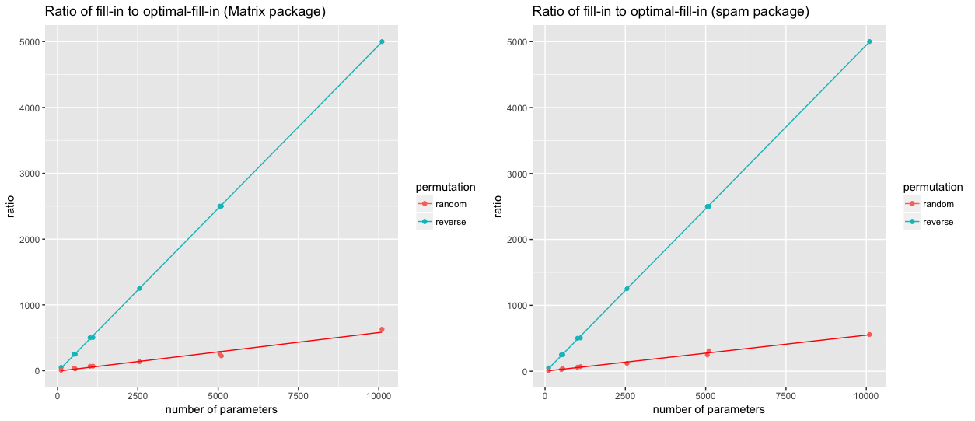
\includegraphics[width=400bp]{Paper_files/figure-latex/plots-1} \end{center}

~~~~~~~~~~~~~~~~~~~~~~~~~~~~~~~~~~~~~ (a)
~~~~~~~~~~~~~~~~~~~~~~~~~~~~~~~~~~~~~~~~~~~~~~~~~~~~~~~~~~~~~~~~~~~~~~~~~~~~
(b)

\begin{center} \smallfont{Figure 3. Fill-in ratio using both Matrix (a) and spam (b) packages}  \end{center}

\vspace{0.6cm}

\midsmallfont{3.4 Future set $F(i,j)$ of Gaussian hierarchical models}
\newline 

For both the \emph{Matrix} and \emph{spam} packages, the optimal fill-in
was obtained when pivot = TRUE for all 3 permutations constructed
(depth-first, random, and reverse), confirming the efficacy of the row
permutation algorithms used by both packages in finding the optimal
configuration for matrix factorization. Both packages are thus robust to
label permutations in the precision matrix. This result can possibly be
explained by the cleanly divided multilevel structure of Gaussian
hierarchical models which makes it easier to order nodes by nested
dissection. Using the \emph{spam} package's \emph{ordering} function,
the permuted precision matrix can be recovered and studied.

It turns out that the permuted precision matrix obtained using the
\emph{ordering} function is labelled in the same manner as the
depth-first permutation (that the labels are not exactly the same is
irrelevant since the positions in the matrix which are non-zero are the
same)! Furthermore, this implies an interesting side result that there
is more than one permutation which results in an optimal fill-in since
the optimal fill-in was also obtained with the lexicographical ordering.

The results in section 3.3 can then be explained by considering the
hierarchical structure together with the future set \(F(i,j)\). Recall
that if all the nodes depend on, or have an edge to, node 1, the fill-in
will be maximal or close to maximal since the set \(F(i,j)\) will never
separate nodes \(i\) and \(j\) regardless of the values of \(i,j\).
Considered simply, this implies that nodes with fewer edges should be
assigned lower numbers and nodes with more edges assigned higher
numbers.

In a Gaussian hierarchical model, this means that the nodes at the
bottom level, which are only connected to its parent, should be given
lower numbers. This is exactly what was done for the lexicographical
ordering as nodes are labelled 1 to \(n\) from the lowest level upwards.
Likewise, this explains why the reversed lexicographical permutation had
the worst fill-in ratio: the nodes which contained more edges in the
higher levels are now given smaller numbers. Equation (2.13) tells us
which entries of the cholesky factor are known to be 0 with certainty.
With a reverseed lexicographical permutation, there is less information
on and more uncertainty on which entries of the cholesky factor are zero
and thus more computations need to be carried out, leading to greater
fill-in. This is because the conditional independence between two nodes
\(i,j\) given the future set \(F(i,j)\) cannot be established if they
are both connected to a node \(k\) such that \(1\leq k<i<j\leq n\).

This also explains why the depth-first permutation is an optimal
permutation since for any node \(i\) where \(1\leq i<n\), the future set
\(F(i,j)\) always contains the nodes which it is connected to. This is
exactly due to the tree-like structure of the graph where each node is
connected only to its parent and children (if available).

Thus, we can use the hierarchical structure to construct labelings for
the precision matrices of Gaussian hierarchical model \emph{a priori} so
that little or no permutation is required before cholesky factorization.
This will lead to computational gains since there is no longer any need
to find a permutation matrix \(\boldsymbol{P}\). Instead, one simply
needs to construct a depth-first labeling as mentioned above.

\vspace{1.0cm}

\midfont{4. Discussion} \newline 

Hierarchical modeling is a practical approach with proven results in
modeling real world data. This paper in particular studied Gaussian
hierarchical models and methods which exploit the sparse conditional
independence structure of such models to conduct scalable and efficient
inference using sparse linear algebra methods. The efficiency of such
methods is highly dependent on the row and column ordering of the
precision matrix to be factorized. The key finding in this paper is that
a depth-first permutation guarantees an optimal permutation of the
precision matrix for Gaussian hierarchical models such that the fill-in
ratio is optimal. This makes the use of permutation algorithms such as
AMD or MMD unnecessary once it is known that the model used is a
Gaussian hierarchical model, saving on computational efficiency. It was
also found that the returned fill-in ratio is also optimal with a
lexicographical ordering. Since the cholesky factor of a
positive-definite matrix is unique, this implies that there is more than
one optimal permutation of the precision matrix which returns minimal
fill-in. A possible area of future research would be to determine if
there are more permutations which also return an optimal fill-in ratio.

This paper illustrates how one can conduct scalable inference on
Gaussian hierarchical models using a naive Gibbs sampler and sparse
linear algebra methods. Other methods of scalable inference which can be
explored include belief propagation (Papaspiliopoulos, Zanella, 2017),
which allows exact draws from high-dimensional distributions at a cost
which scales linearly in the number of parameters and data, at the
expense of higher variable node dimensions.

\newpage

\midfont{Appendix} \newline \newline \newline
\midsmallfont{A1. Extension to 3-level model} \newline 

For a 3-level model, we retain equations (2.1) to (2.3). However, we add
an aditional level and a modified observation level.

\[\beta_{ijk} \;|\; \beta_{ij} \sim N( \beta_{ij}, \tau_c)\]

\[y_{ijk} \;|\; \beta_{ijk} \sim N( \beta_{ijk}, \sigma^2)\]
\newline \newline \newline

\midsmallfont{A2. Calculating precision matrix entries} \newline 

\[
\begin{aligned}
P(\boldsymbol{\beta} \; | \;\boldsymbol{y}) &= \frac{P(\boldsymbol{y}\;|\;\boldsymbol{\beta}) P(\boldsymbol{\beta})}{P(\boldsymbol{y})}  \\ 
&\propto P(\boldsymbol{y}\;|\; \boldsymbol{\beta}) P(\boldsymbol{\beta}) \\
&=  P(\beta) \prod_{i} P(\beta_i \;|\; \beta) \prod_{i,j}P(\beta_{ij} \;|\; \beta_i) \prod_{i,j,k}P(\beta_{ijk} \;|\; \beta_{ij}) \prod_{i,j,k}P(y_{ijk} \;|\; \beta_{ijk})\\
&\propto \exp\{-\frac{1}{2\sigma^2}\ \sum_{i,j,k} (y_{ijk}-\beta_{ijk})^2 - \frac{1}{2\tau_c}\sum_{i,j,k} (\beta_{ijk}-\beta_{ij})^2 -\frac{1}{2\tau_b} \sum_{i,j} (\beta_{ij}-\beta_{i})^2 - \frac{1}{2\tau_a} \sum_i (\beta_{i}-\beta)^2  - \\ &\frac{1}{2\tau}(\beta - \mu)^2 \} \\
&\propto \exp\{-\frac{1}{2} \boldsymbol{\beta^{T}} Q \boldsymbol{\beta}\}
\end{aligned}
\]

By expanding out the squared terms and rearranging them, we can deduce
the terms of the posterior precision matrix Q. If we assume a flat
prior,

\[
\begin{aligned}
\exp\{-\frac{1}{2} \boldsymbol{\beta}^{T} \boldsymbol{Q} \boldsymbol{\beta} \} \propto \exp\{-\frac{1}{2}(\sum_{i,j}(\frac{\beta_{ij}^2}{\sigma^2} + \frac{\beta_{ij}^2}{\tau_b}+\frac{\beta_{i}^2}{\tau_b} - \frac{2 \beta_{ij}\beta_i}{\tau_b}) + \sum_i( \frac{\beta_i^2}{\tau_a} + \frac{\beta^2}{\tau_a} - \frac{2\beta_i\beta}{\tau_a})  )\}
\end{aligned}
\]

For example, the conditional precision of \(\beta_{ij}\) is
\(\frac{1}{\sigma^2} + \frac{1}{\tau_b}\), and the conditional precision
between \(\beta_{ij}\) and \(\beta_i\) is \(- \frac{1}{\tau_b}\). To
better illustrate, for \(I=3\) and \(J=4\), the constructed precision
matrix is shown below: \newline \newline
\[
\bordermatrix{
  ~       & \text{$\beta_{11}$} & \text{$\beta_{12}$} & \text{$\cdots$} & \text{$\beta_{1I}$} & \text{$\cdots$} & \text{$\beta_{IJ}$} & \text{$\beta_{1}$} & \text{$\cdots$} & \text{$\beta_{I}$} & \text{$\beta$} \cr
  \text{$\beta_{11}$}   & \frac{1}{\text{$\sigma^2$}} + \frac{1}{\text{$\tau_b$}} & 0 & \text{$\cdots$} & 0 & \text{$\cdots$} & 0 & -\frac{1}{\text{$\tau_b$}} & \text{$\cdots$} & 0 & 0 \cr
  \text{$\beta_{12}$}   & 0 & \frac{1}{\text{$\sigma^2$}} + \frac{1}{\text{$\tau_b$}} & \text{$\cdots$} & 0 & \text{$\cdots$} & 0 & -\frac{1}{\text{$\tau_b$}} & \text{$\cdots$} & 0 & 0 \cr
  \text{$\vdots$}   & \text{$\vdots$}   & \text{$\vdots$} & \text{$\ddots$} & \text{$\vdots$} & \text{$\ddots$} & \text{$\vdots$} & \text{$\vdots$} & \text{$\ddots$} & \text{$\vdots$} & \text{$\vdots$}  \cr
  \text{$\beta_{1I}$}   & 0 & 0 & \text{$\cdots$} & \frac{1}{\text{$\sigma^2$}} + \frac{1}{\text{$\tau_b$}} & \text{$\cdots$} & 0 & -\frac{1}{\text{$\tau_b$}} & \text{$\cdots$} & 0 & 0 \cr
  \text{$\vdots$}   & \text{$\vdots$}   & \text{$\vdots$} & \text{$\ddots$} & \text{$\vdots$} & \text{$\ddots$} & \text{$\vdots$} & \text{$\vdots$} & \text{$\ddots$} & \text{$\vdots$} & \text{$\vdots$}  \cr
  \text{$\beta_{IJ}$} & 0 & 0 & \text{$\cdots$} & 0 & \text{$\cdots$} & \frac{1}{\text{$\sigma^2$}} + \frac{1}{\text{$\tau_b$}} & 0 & \text{$\cdots$} & -\frac{1}{\text{$\tau_b$}} & 0 \cr
  \text{$\beta_{1}$} & -\frac{1}{\text{$\tau_b$}} & -\frac{1}{\text{$\tau_b$}} & \text{$\cdots$} & -\frac{1}{\text{$\tau_b$}} & \text{$\cdots$} & 0 & \frac{1}{\tau_a} + \sum_{j} \frac{1}{\tau_b} & \text{$\cdots$} & 0 & -\frac{1}{\text{$\tau_a$}} \cr
  \text{$\vdots$}   & \text{$\vdots$}   & \text{$\vdots$} & \text{$\ddots$} & \text{$\vdots$} & \text{$\ddots$} & \text{$\vdots$} & \text{$\vdots$} & \text{$\ddots$} & \text{$\vdots$} & \text{$\vdots$}  \cr
  \text{$\beta_{I}$}  & 0 & 0 & \text{$\cdots$} & 0 & \text{$\cdots$} & -\frac{1}{\text{$\tau_b$}} & 0 & \text{$\cdots$} & \frac{1}{\tau_a} + \sum_{j} \frac{1}{\tau_b} & -\frac{1}{\text{$\tau_a$}} \cr
  \text{$\beta$} & 0 & 0 & \text{$\cdots$} & 0 & \text{$\cdots$} & 0 & -\frac{1}{\text{$\tau_a$}} & \text{$\cdots$} & -\frac{1}{\text{$\tau_a$}}  & \sum_i \frac{1}{\tau_a} \cr
}
\]

\vspace{1.0cm}

\midsmallfont{A3. Proof for equation (2.12):} \newline 

Using the fact that
\(x \; \perp \; y \;|\; z \iff P(x,y,z) = f(x,z) g(y,z)\) for some
functions \(f\) and \(g\) (Rue, Held, 2002), let
\(\mathbf{x} = (x_i, x_j, \mathbf{x}_{-\{ij\}})\), and setting the mean
to be 0 without loss of generality, we have that for \(i \neq j\):

\[
\begin{aligned}
P(x_i, x_j, \mathbf{x_{-\{ij\}}}) &= f(x_i, \mathbf{x_{-\{ij\}}}) g(x_j,\mathbf{x_{-\{ij\}}})\\
P(x_i, x_j, \mathbf{x_{-\{ij\}}}) &\propto \exp\{-\frac{1}{2} \sum_{k,l} x_k Q_{kl} x_l\} \\
&\propto \exp\{-\frac{1}{2}x_i x_j (Q_{ij} + Q_{ji}) -\frac{1}{2}\sum_{\{k,l\} \neq \{i,j\}} x_k Q_{kl} x_l\} \\
\end{aligned}
\] Since in this case, it is already assumed that
\(x_i \; \perp \; x_j \;|\; \mathbf{x_{-\{ij\}}}\), it follows that
\(Q_{ij} = Q_{ji} = 0\). \newline \newline \newline

\midsmallfont{A4. Proof for equation (2.13):} \newline 

Let \(\boldsymbol{x}\) be a GMRF with respect to the labelled graph G,
with mean \(\boldsymbol{\mu}\) and positive-definite precision matrix
\(\boldsymbol{Q}\). Let \(\boldsymbol{L}\) be the Cholesky triangle of
\(\boldsymbol{Q}\). Then for \(i \in V\),

\[
\begin{aligned}
E(x_i | \boldsymbol{x}_{(i+1):n}) &= \mu_i − \frac{1}{L_ii} \sum_{j=i+1}^n L_{ji}(x_j − \mu_j) \;\;\; - (a.2)\\ 
Prec(x_i | \boldsymbol{x}_{(i+1):n}) &= L^2_{ii} \;\;\; - (a.3)
\end{aligned}
\] Assume for simplicity that \(\boldsymbol{\mu} = 0\) and fix
\(1 \leq i < j \leq n\), then:

\[
\begin{aligned}
P(\boldsymbol{x}_{i:n}) &\propto \exp \left( -\frac{1}{2} \sum_{k=i}^n L_{kk}^2 \; \left(x_k + \frac{1}{L_{kk}} \sum_{j = k+1}^n L_{jk} x_j\right)^2 \right) \\
&= \exp \left(-\frac{1}{2}\boldsymbol{x}_{i:n}^T \boldsymbol{Q}^{(i:n)} \boldsymbol{x}_{i:n} \right) \;\;\; - (a.4)
\end{aligned}
\]

where \(\boldsymbol{Q}^{i:n} = L_{ii} L_{ji}\). Using equation (2.12),
it follows that:
\[x_i \; \perp \; x_j \;|\; \boldsymbol{x}_{F(i,j)} \iff L_{ii}L_{ji}=0 \;\;\; - (a.5)\]
which is equivalent to equation (2.13) since \(L_{ii}>0\) because the
precision matrix is positive-definite. \newline \newline \newline

\midsmallfont{A5. Markov properties of GMRF} \newline 

This section is written with reference to Theorem 2.4 in Rue and Held
(2002). From equation (2.12), a GMRF represented by the graph
\(G = (V,E)\) is defined by the non-zero pattern in the precision matrix
\(\boldsymbol{Q}\), since that tells you which nodes have edges to which
other nodes. It turns out that for a GMRF, the pairwise Markov property
defined in equation (2.11) is equivalent to the global Markov property:

\[\boldsymbol{x}_A \; \perp \; \boldsymbol{x}_B \;|\; \boldsymbol{x}_{C} \;\;\; - (a.1) \]
for all disjoint sets \(A, B\), and \(C\) where \(C\) separates \(A\)
and \(B\), and \(A\) and \(B\) are non-empty. \newline \newline \newline

\midsmallfont{A6. Full conditionals for Gibbs sampler } \newline 

Adopting the notation from Roberts \& Zanella (2017),
\[\beta. = \frac{\sum_i\beta_i}{I}\]

\[\beta_{^.j} = \frac{\sum_i\beta_{ij}}{I}, \; \beta_{^{..}k} = \frac{\sum_{i,j}\beta_{ijk}}{IJ}\]
and so on. Note that the following derivation for the full conditionals
of the Gibbs sampler are for a centered parametrization with a flat
prior.

Assuming that \(\mu=0\), the full conditional is proportional to the
posterior density of the coefficients. Since we are only concerned with
\(\beta\), we can ignore all factors which do not contain \(\beta\):

\[
\begin{aligned}
P(\beta \;|\; \beta_{1:I}, \; \beta_{1:I,1:J}, \; y^*) &= \frac{P(\beta^* \;|\; y^*)}{P(\beta_{1:I},\; \beta_{1:I, 1:J}\;|\; y^*)} \\
&\propto \exp \{-\frac{1}{2\sigma^2}\ \sum_{i,j} (y_{ij}-\beta_{ij})^2 - \frac{1}{2\tau_b}\sum_{i,j} (\beta_{ij}-\beta_{i})^2 -\frac{1}{2\tau_a} \sum_{i} (\beta_{i}-\beta)^2 - \frac{1}{2\tau}(\beta - \mu)^2 \}\\
&\propto \exp \{ -\frac{1}{2\tau_a} \sum_i (\beta^2 -2\beta_i\beta) - \frac{1}{2\tau}\beta^2\}
\end{aligned}
\]

To generate samples from a Gaussian, all we need are the first and
second moments. By expanding and manipulating the above, we can obtain a
form to read off the mean and variance of the full conditional.

\[
\begin{aligned}
\exp \{-\frac{1}{2\tau_a} \sum_i (\beta^2 -2\beta_i\beta) - \frac{1}{2\tau}\beta^2\} &= \exp \{-\frac{1}{2} \frac{\tau I \beta^2 - 2\tau\beta\sum_{i}\beta_i + \tau_a \beta^2}{\tau_a\tau}\} \\
&= \exp \{-\frac{1}{2} \frac{(\tau+ \frac{\tau_a}{I}) \beta^2 - 2\tau\beta \beta.} {\frac{\tau_a\tau}{I}}\}\\ 
&= \exp \{-\frac{1}{2} \frac{\beta^2 - 2\beta \beta. \frac{\tau}{\frac{\tau_a}{I}+\tau}} { \frac{\frac{\tau_a\tau }{I}} {\frac{\tau_a}{I}+\tau}}\}\\
&\propto \exp \{-\frac{1}{2} \frac{(\beta - \beta. \frac{\tau}{\frac{\tau_a}{I}+\tau})^2} { \frac{\frac{\tau_a\tau }{I}} {\frac{\tau_a}{I}+\tau}}\} 
\end{aligned}
\]

where \(\beta. = \frac{\sum_i\beta_i}{I}\). From this, we can deduce the
mean and variance of the posterior distribution of \(\beta\).

\[\beta \;|\; \beta_{1:I}, \;\beta_{1:I,1:J}, \boldsymbol{y} \sim N(\frac{\beta.\tau}{\frac{\tau_a}{I}+\tau}, \frac{\frac{\tau_a \tau}{I}}{\frac{\tau_a}{I}+\tau})\]
In the same way, the full conditionals for the other parameters can be
derived.

\[\beta_i \;|\; \beta, \;\beta_{1:I,1:J}, \boldsymbol{y} \sim N(\frac{(\frac{\tau_b}{J} \beta + \tau_a \beta_{i\cdot})}{\tau_a + \frac{\tau_b}{J}},  \frac{\frac{\tau_a\tau_b }{J}} {\frac{\tau_b}{J}+\tau_a})\]

\[\beta_{ij} \;|\; \beta, \;\beta_{1:I}, \boldsymbol{y} \sim N(\frac{\beta_i \sigma^2}{\tau_b + \sigma^2},  \frac{\tau_b \sigma^2}{\tau_b + \sigma^2})\]

\newpage

\midfont{References} \newline 

Alan George and Joseph W. Liu, 1981. Computer Solution of Large Sparse
Positive Definite. Prentice Hall Professional Technical Reference.

Alan George and Joseph W. Liu, 1989. The Evolution of the Minimum Degree
Ordering Algorithm. SIAM Review, 31:1, (March 1989), 1-19.

Andrew Gelman, 2006, Multilevel (Hierarchical) Modeling: What It Can and
Cannot Do, Technometrics, 48:3, 432-435.

David Draper, 1995. Inference and Hierarchical Modeling in the Social
Science. \emph{Journal of Educational and Behavioral Statistic} 20:2,
115-147.

Esmond G. Ng and Barry W. Peyton. 1993. Block sparse Cholesky algorithms
on advanced uniprocessor computers. SIAM J. Sci. Comput. 14:5,
(September 1993), 1034-1056.

Giacomo Zanella and Gareth O. Roberts, 2017. Analysis of the Gibbs
Sampler for Gaussian hierarchical models via multigrid decomposition.
arXiv:1703.06098{[}stat.CO{]}.

Havard Rue and Leonhard Held, 2005. Gaussian Markov Random Fields:
Theory and Applications (Monographs on Statistics and Applied
Probability), Chapter 2. Chapman \& Hall/CRC.

Johannes Textor, Benito van der Zander, Mark K. Gilthorpe, Maciej
Liskiewicz, George T.H. Ellison, 2016. Robust causal inference using
directed acyclic graphs: the R package `dagitty'. \emph{International
Journal of Epidemiology} 45(6):1887-1894.

Martin Maechler and Douglas Bates, 2006. 2nd Introduction to the Matrix
Package, R Core Development Team. Accessed on:
\url{https://stat.ethz.ch/R-manual/R-devel/library/Matrix/doc/Intro2Matrix.pdf}.

Omiros Papaspiliopoulos and Giacomo Zanella, 2017. A note on MCMC for
nested multilevel regression models via belief propagation.
arXiv:1704.06064 {[}stat.CO{]}

Patrick R. Amestoy, Timothy A. Davis, and Iain S. Duff, 1996. An
Approximate Minimum Degree Ordering Algorithm. SIAM J. Matrix Analysis
\& Applic., 17:4, 886-905.

Reinhard Furrer and Stephan R. Sain, 2010. spam: A Sparse Matrix R
Package with Emphasis on MCMC Methods for Gaussian Markov Random Fields.
Journal of Statistical Software, 36, 1-25.

Timothy A. Davis, 2009. User guide for CHOLMOD: a sparse Cholesky
factorization and modification package.
\url{http://citeseerx.ist.psu.edu/viewdoc/download?doi=10.1.1.220.238\&rep=rep1\&type=pdf}.
Accessed 2018-06-05.


\end{document}
